\documentclass[9pt,twocolumn,twoside]{../../styles/osajnl}
\usepackage{fancyvrb} \journal{i524}

\title{An Overview of Apache Spark}

\author[1]{Snehal Chemburkar}
\author[1]{Rahul Raghatate}

\affil[1]{School of Informatics and Computing, Bloomington, IN 47408,
  U.S.A.}

\affil[*]{Corresponding authors: snehchem@iu.edu, rraghtate@iu.edu}

\dates{paper-1, \today}

\ociscodes {Spark, RDDs, DAG, Spark SQL, MLlib, GraphX, I524}

% replace this with your url in github/gitlab
\doi{\url{https://github.com/cloudmesh/sp17-i524/raw/master/paper2/S17-IO-2006/report.pdf}}


\begin{abstract}
Apache Spark, developed at UC Berkeley AMPLAB, is a high performance
framework for analyzing large datasets \cite{article-spark-1}. The
main idea behind the development of Spark was to create a generalized
framework that could process diverse and distributed data as opposed
to MapReduce which only support batch processing of data. Spark has
multiple libraries built on top of its core computational engine which
help process diverse data. This paper will discuss the Spark runtime
architecture, its core and libraries. \newline
\end{abstract}

\setboolean{displaycopyright}{true}

\begin{document}

\maketitle

\section{Introduction}

Spark is an open source, easy-to-use distributed cluster computing
engine for processing the different types of data available these
days. Spark provides a generalized framework which can efficiently
process MapReduce jobs (batch processing) as well as iterative
algorithms, interactive data mining and streaming analytics. Iterative
algorithms include many machine learning algorithms which iterate over
the same dataset to optimize a parameter. Interactive data mining
refers to executing ad-hoc queries to explore the dataset.

MapReduce can process iterative algorithms by splitting each iteration
into a separate MapReduce job. Each job must then read data from a
stable storage and write it back to a stable storage at each
intermediate step. This repeated access to the stable storage systems
like physical disks or HDFS increases the processing time while
reducing efficiency of the system. For interactive data mining in
Hadoop, the data is loaded in memory across a cluster, and queried
repeatedly. Each query is executed as separate MapReduce job which
reads data from the HDFS or hard drives thus incurring significant
latency (tens of seconds) \cite{paper-zaharia}.  Spark is specialized
to make data analysis faster in terms of data write speed as well as
program execution. It supports in-memory computations which enables
faster data querying compared to disk-based systems like Hadoop.

Spark is implemented in Scala, a high level programming language that
runs on JVM. It makes programming easier by providing a clean and
concise API for Scala, Java and Python \cite{paper-zaharia}. Spark
also provides libraries that allow for iterative, interactive,
streaming and graph processing. Spark SQL library provides for
interactive data mining in Spark. MLlib provides Spark with machine
learning algorithms required for iterative computations. Similarly
Spark streaming and GraphX libraries enables Spark to process
real-time and graph processing data respectively. These high level
components required for processing the diverse workloads such as
structured or streaming data are powered by the Spark Core. The
distribution, scheduling and monitoring of clusters is done by the
Spark Core.

The Spark Core and it's higher level libraries are tightly integrated
meaning when updates or improvements are implemented in the Spark core
help improve the Spark libraries as well. Tight integration also makes
it easier to write applications combining different workloads. This is
explained nicely in the following example. One can build an
application using machine learning libraries to process real time data
from streaming sources and analysts can simultaneously access the data
using SQL also in real time.  In this example three different
workloads namely SQL, streaming data and machine learning algorithms
can be implemented in a single system which is a requirement in
today’s age of big data.

\section{Spark Components}

Figure \ref{fig:spark-stack} depicts the various building blocks of
the Spark stack. The Spark Core is computational engine which performs
the task scheduling, distribution, and cluster monitoring
tasks. Resilient Distributed Datasets(RDD) \cite{paper-RDD} and
Directed Acyclic Graphs(DAG) are two important concepts in Spark. RDDs
are a collection of read-only Java or Python objects parallelized
across a cluster. DAGs, as the name suggests are directed graphs with
no cycles. The libraries or packages supporting the diverse workloads,
built on top of the Spark Core, include Spark SQL, Spark Streaming,
MLlib (machine learning library) and GraphX. The Spark Core runs atop
cluster managers which are covered in section 4.

\begin{figure}[htbp]
\centering
\fbox{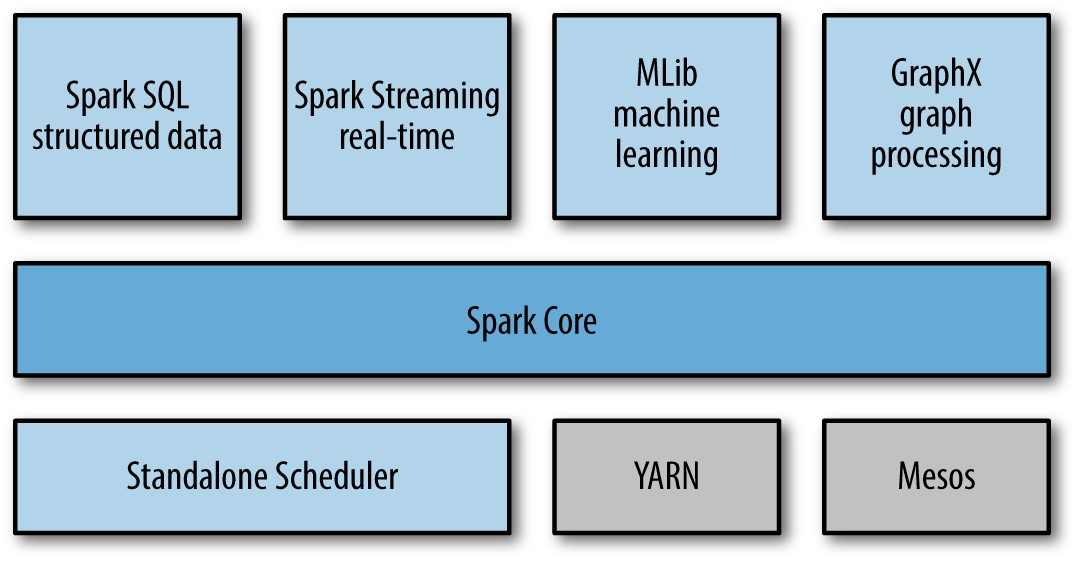
\includegraphics[width=\linewidth]{images/Spark-Components}}
\caption{Spark Components \cite{book-spark}.}
\label{fig:spark-stack}
\end{figure}

\subsection{Spark Core}

Spark Core is the foundation framework that provides basic I/O
functionality, distributed task scheduling and dispatching
\cite{article-spark-1}.
\subsection{Resilient Distributed Datasets(RDD)}
Resilient Distributed Datasets(RDD) \cite{paper-RDD} are Spark's
primary abstraction, which are a fault-tolerant collection of elements
that can be operated in parallel. RDDs are immutable once they are
created but they can be transformed or actions can be performed on
them \cite{article-spark-1}. Users can create RDDs through external
sources or by transforming another RDD. Transformations and Actions
are the two types of operations supported by RDDs.
\begin{itemize}
\item \textit{Transformations}: Since RDDs are immutable, the
  transformations return a new RDD and not a single value. RDDs are
  lazily evalutated i.e they are not computed immediately when a
  transformation command is given. They wait till an action is
  received to execute the commands. This is called Lazy
  evaluation. Examples of transformation functions are map, filter,
  ReduceByKey, FlatMap and GroupByKey \cite{article-spark-1}.
\item \textit{Actions} are operations that result in a return value
  after computation or triggers a task in response to some
  operation.Some Action operations are first, take, reduce, collect,
  count, foreach and CountByKey \cite{article-spark-1}.
\end{itemize}
RDDs are ephemeral disk, which means they do not persist
data. However, users can explicitly persist RDDs to ease data
reuse. Traditional distributed computing systems provide fault
tolerance through checkpoint or data replication. The transformations
used to build a data set are logged and can be used to rebuild the
original data set through its lineage \cite{paper-RDD}. If one of the
RDD fails, it has enough information about of its lineage so as to
recreate the dataset from other RDDs, thus saving cost and time.
\subsection{Directed Acyclic Graph(DAG)}
Directed Acyclic Graph(DAG), which supports acyclic data flow,
"consists of finitely many vertices and edges, with each edge directed
from one vertex to another, such that there is no way to start at any
vertex v and follow a consistently-directed sequence of edges that
eventually loops back to v again \cite{wiki-DAG}." When we run any
application in Spark, the driver program converts the transformations
and actions to logical directed acyclic graphs(DAG). The DAGs are then
converted to physical execution plans with a set of stages which are
distributed and bundled into tasks. These tasks are distributed among
the different worker nodes for execution.

\subsection{Spark SQL}
Spark SQL \cite{book-spark} is a library built on top of the Spark
Core to support querying structured data using SQL or Hive Query
Language. It allows users to perform ETL (Extract, Transform and Load)
operations on data from various sources such as JSON, Hive Tables and
Parquet. Spark SQL provides developers with a seamless intermix of
relational and procedural API, rather than having to choose between
the two.  It provides a DataFrame API that enables relational
operations on both the in-built collections as well as external data
sources. Spark SQL also provides a novel optimizer called Catalyst, to
support the different data sources and algorithms found in big data
\cite{paper-sparksql}.

\subsection{Spark Streaming}
Spark Streaming \cite{book-spark} library enables Spark to process
real time data. Examples of streaming data are messages being
published to a queue for real time flight status update or the log
files for a production server. Spark's API for manipulating data
streams is very similar to the Spark Core’s RDD API. This similarity
makes it easier for users to move between projects with stored and
real-time data as the learning curve is short.  Spark Streaming is
designed to provide the same level of fault tolerance, throughput and
scalability as the Spark Core.

\subsection{MLlib}
MLlib \cite{book-spark} is a rich library of machine learning
algorithms for, which can be accessed from Java, Scala as well as
Python. It provides Spark with various machine learning algorithms
such as classification, regression, clustering, and collaborative
filtering. It also provides machine learning functionality such as
model evaluation and data import. The common machine learning
algorithms include K-means, navie Bayes, logistic regression,
principal component analysis and so on. It also provides basic
utilities for feature extractions, optimizations and statistical
analysis to name a few \cite{article-mllib}.

\subsection{GraphX}

GraphX is a graph processing framework built on top of Spark. It
introduces the Resilient Distributed Property Graph, which is directed
multi-graph having properties attached to each edge and vertex. GraphX
includes a set of operators like aggregateMessages, subgraph and
joinVertices, and optimized variant of Pregel API. It also includes
builders and graph algorithms to simplify graph analytics tasks
\cite{article-spark-1}.

\section{Runtime Architecture}

The runtime architecture of Spark, illustrated in Figure
\ref{fig:spark-runtime}, consists of a driver program, a cluster
manager, workers or executors and the HDFS (Hadoop Distributed File
System) \cite{article-spark-1}.  Spark uses a master/slave
architecture in which the driver program is the master whereas the
worker nodes or executors are the slaves. The driver runs the main()
method of the user program which creates the SparkContext, the RDDs
and performs transformations and actions \cite{book-spark}.

\begin{figure}[htbp]
\centering
\fbox{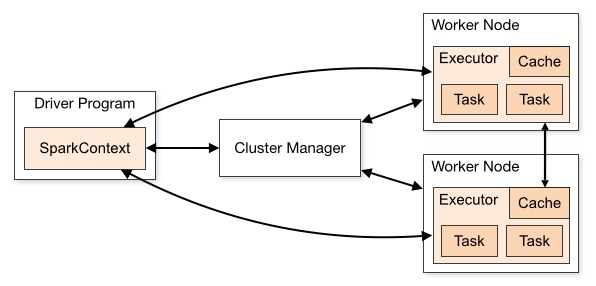
\includegraphics[width=\linewidth]{images/cluster-overview.jpg}}
\caption{Spark Architecture \cite{www-spark-cluster}.}
\label{fig:spark-runtime}
\end{figure}

When we launch an application using the Spark Shell it creates a
driver program which in turn initializes the SparkContext. Each Spark
application has its own SparkContext object which is responsible for
the entire execution of the job. The SparkContext object then connects
to cluster manager to request resources for its workers. The cluster
manager provide executers to worker nodes, which are used to run the
logic and also store the application data. The driver will send the
tasks to the executors based on the data placement. The executors
register themselves with the driver, which helps the driver keep tabs
on the executors. Driver can also schedule future tasks by caching or
persisting data.

\section{Deployment Modes}

Spark can be deployed in local and clustering modes. The local mode of
Spark runs a single node. In clustering mode, Spark can connect to any
of the following cluster managers - standalone cluster manager, YARN
or Mesos - explained in the following sections.

\subsection{Standalone}
Standalone cluster manager is the built-in cluster manager provided by
spark in its default distribution. To run your Spark application in a
standalone clustered environment, make sure that Spark must be
installed on all nodes in the cluster. Once Spark is available on all
nodes, follow the steps given in Spark documentation to start the
master and workers. The master server has a web UI which is located at
\texttt{http://localhost:8080/} by default. This UI will give
information regarding the number of CPUs and memory allocated to each
node. The Standalone Master acts as the resource manager and allocates
resources to the Spark application based on the number of cores. Spark
standalone mode is not very popular in production environments due to
reliability issues \cite{www-clusters}.

\subsection{YARN}
YARN (Yet Another Resource Negotiator) is the resource manager in
Hadoop ecosystem. Like the Standalone cluster master, the YARN
ResourceManager decides which applications get to run executor
processes, where they run it and when they run it. The YARN
NodeManager is the slave service that runs on every node and runs the
executor processes. This service also helps monitor the resource
consumption at each node. YARN is the only cluster manager for Spark
that provides security support \cite{www-clusters}. To run Spark on
YARN, Spark distribution with YARN support must be downloaded from the
Apache Spark download page.

\subsection{Apache Mesos}
Apache Mesos is an open source distributed systems kernel, using
principles similar to the Linux kernel but at a different level of
abstraction. This kernel provides Spark with APIs for resource
management and scheduling across the cluster and runs on each node in
the cluster. While scheduling tasks, Mesos considers the other
frameworks that may coexist on the same cluster. The advantage of
deploying Spark with Apache Mesos include dynamic partitioning between
Spark and other frameworks and scalable partitioning between multiple
instances of Spark. Installation of Mesos for Spark is similar to its
installation for use by any other frameworks. You can either download
Mesos release from its source or from the binaries provided by third
party projects like Mesosphere \cite{www-clusters}.

\section{Easy Installation Using Pre-built Packages}
To run Spark on your Windows, Linux or Mac systems you need to have
Java 7+ installed on your system. To verify if you have java installed
on your Linux machine type \texttt{java -version} command in the
terminal.  If you do not have Java installed on your system you can
download it from the Oracle website \cite{www-oracle}. The environment
variable \texttt{PATH} or \texttt{JAVA\_}\texttt{HOME} must be set to
point to the Java installation.  Now that the Java prerequisite is
satisfied, go to the download page of Apache Spark, select the 2.1.0
(latest version as on $26^{th}$ March 2017) version of Spark, select
the pre-built Hadoop 2.7 package and download the
\texttt{spark-2.1.0-bin-hadoop2.7.tgz} file. Then, go to the terminal
and change the directory folder to where the file is located and
execute the following command to unzip the file
\begin{verbatim}
tar -xvf spark-2.1.0-bin-hadoop2.7.tgz -C -/
\end{verbatim}
This will create a folder \texttt{spark-2.1.0-bin-hadoop2.7} in that
directory. Move this folder to the \texttt{/usr/local/spark} using
command \texttt{mv spark-2.1.0-bin-hadoop2.7 /usr/local/spark} To set
the environment variable for Spark, open the \texttt{.bashrc} file
using command \texttt{sudo nano ~/.bashrc} and add the following lines
at the end of this file.
\begin{verbatim}
export SPARK_HOME = /usr/local/spark export PATH = $PATH:
 $SPARK_HOME/bin
\end{verbatim}
Go back to your home directory and execute \texttt{.bashrc} using
command \texttt{. .bashrc} for the changes to take effect. This change
can be verified by executing command \texttt{echo \$PATH}. The
\texttt{PATH} variable should now reflect the path to the spark
installation. To verify that Spark is installed correctly, execute
command \texttt{\$spark-shell} in the terminal. It will display the
Spark version and then enter the Scala prompt.

\section{Building Spark based applications}
The first step to start building Spark based applications is exploring
the data in Spark Local Mode and developing a prototype. Spark local
mode runs on a single node and can be used by developers to learn
Spark by building a sample application that leverages the
functionalities of Spark API. The developer can use Spark Shells like
Scala REPL or PySpark to develop a quick prototype. It can then be
packaged as a Spark application using Maven or Scala Build Tool(SBT)
\cite{www-hortonworks}.  The second step involves deploying the Spark
application to production. To achieve this, the developer will fine
tune the prototype by running it against a larger dataset. This
involves running Spark in cluster mode on YARN or Mesos. Thus the
prototype application created in the local mode of Spark will now be
submitted as a Spark job to the production cluster
\cite{www-hortonworks}.

\section{Performance Monitoring Tools}
Spark provides a web interface to monitor its applications. By
default, each SparkContext launches a webUI, at port 4040. This UI
displays the the memory usage statistics, list of scheduler stages and
tasks, environmental information and information about the executors.
This interface can be access by opening
\texttt{http://<driver-node>:4040} in the web browser.  If multiple
instances of SparkContext are running on the same machine, then they
will bind to successive ports beginning with 4040 (4041, 4042, 4043,
$\ldots$).  This information is only available for the life of the
application. To view this information after the life of the
application, set \texttt{spark.eventLog.enabled} to true before
starting the application.  This will configure Spark to store the
event log to persistent storage \cite{www-spark-ui}.

A REST API which enables the metrics to be extracted in JSON format,
making it easier for developers to create visualizations and
monitoring tools for Spark \cite{www-spark-ui}.  These metrics can
also be extracted as HTTP, JMX, and CSV files by configuring the
metric system in the configuration file present at
\texttt{\$SPARK\_HOME/conf/metrics.properties}. In addition to these,
external tools like Ganglia, dstat, iostat, iotop, jstack, jmap, jmap,
and jconsole can also be monitor Spark performance
\cite{www-spark-ui}.

\section{Use Cases}

In its early days, Spark was adopted in production systems by
companies like Yahoo, Conviva, and ClearStory for personlization,
analytics, streaming and interactive processing. These use cases are
explained in further paragraphs.  \textit{Yahoo News Personalization}:
This project implements machine learning algorithms on Spark to
improve news personalization for their visitors. Spark runs on Hadoop
Yarn to use existing data and clusters. In order to achieve
personalization, the system will learn about users’ interests from
their clicks on the web page. It also needs to learn about each news
and categorize it. The SparkML algorithm written for this project was
120 lines of Scala code as compared to the 15,000 lines of C++ code
used previously \cite{www-spark-datanami}.

\textit{Yahoo Advertisement Analytics}: In this project Yahoo
leverages Hive on Spark to query and visualize the existing BI
analytic data that was stored in Hadoop. Since Hive on Spark (Shark)
uses the standard Hive server API, any tools that can be plugged into
Hive, will automatically work with Shark. Thus visualization tools
like Tableau that are compatible with Hive can be used with Shark to
interactively query and view their ad visit data
\cite{www-spark-datanami}.

\textit{Monitor Network Conditions in Real-time}: Conviva is a video
streaming company with a huge video feed database. To ensure quality
service, it requires pretty sophisticated technology to be applied
behind the scenes to ensure high quality service. With the increase in
internet speeds, people's tolerance towards buffering or delays has
plummeted. To keep up with the rising expectations of high quality and
speed for streaming videos, Conviva implemented Spark Streaming to
learn about the network conditions in real-time. This information is
then feed to the video player running on the user's laptop to optimize
the video speeds \cite{www-spark-datanami}.

\textit{Merge Diverse Data Sources}: ClearStory develops data
analytics software with speciality in data harmonization. To merge
data from internal and external sources for its business users, they
turned to Spark, which is one of the core components of their
interactive and real-time product \cite{www-spark-datanami}.

\textit{Credit Card Fraud Detection}: Using Spark Streaming on Hadoop,
banks can detect fraudulent transactions in real-time. The incoming
transactions are verified in real-time against a known database of
fraudulent transactions. Thus a match against the known database will
alert the call center personnel to instantly verify the transaction
with the credit card owner. The authentic transactions are stored to
the Hadoop file system where they are used to continuously update the
model using deep machine learning techniques
\cite{www-spark-linkedin}.

\textit{Network Security}: Spark can be used to examine network data
packets for traces of malicious activity. Spark streaming checks the
data packets against known threats and then forwards the unmatched
data packets to the storage devices where it is further analyzed using
the GraphX and MLlib libraries \cite{www-spark-linkedin}.

\textit{Genomic Sequencing}: Genomic companies are leveraging the
power of Spark to align chemical compounds with genes. Spark has
reduced the genome data processing time from a few weeks to a couple
of hours \cite{www-spark-linkedin}.

These are few of the real-world use cases of Spark. Real-world
applications of Spark that incorporate MongoDB are Content
Recommendations, Predictive Modeling, Targeted Ads and Customer
Service \cite{www-spark-mongodb}.

\section{When Not to Use Spark}
Apache Spark is not the most suitable data analysis engine when it
comes to processing (1) data streams where latency is the most crucial
aspect and (2) when the available memory for processing is
restricted. In cases where latency is the most crucial aspect we can
get better results using Apache Storm. Since Spark maintains it's
operations in memory, Hadoop MapReduce should be preferred, when
available memory is restricted \cite{article-spark-persp}.

\section{Educational Resources}
 The Apache Spark website has a detailed documentation on the how to
 get started with Spark \cite{www-apache-spark}. It explains the
 concepts and shows examples to help us familiarize with Spark.

\section{Licensing}
Apache Spark is an open-source software licensed under the Apache
License 2.0 \cite{www-apache-lic}. Under this license, it is free to
download and use this software for personal or commercial purposes. It
forbids the use of marks owned by the Apache Software Foundation in a
way that might imply that you are the creator of the Apache
Software. It requires that you copy the license in any redistribution
made by you which includes the Apache Software. You need to provide
acknowledgement for any distributions that include the Apache Software
\cite{www-apache-lic}.

\section{Conclusion}
Apache Spark is an open source cluster computing framework, which has
emerged as the next generation big data processing engine surpassing
Hadoop MapReduce. Spark facilitates in-memory computations which help
execute the diverse workloads efficiently. It's ability to join
datasets across various diverse data sources is one of it's major
attributes. As mentioned in the previous section, Apache Spark is
suitable for almost any kind of big data analysis except for the
following scenarios: (1) where latency is the most crucial aspect and
(2) when the available memory for processing is restricted. Spark
finds place in almost all types of big data analysis projects, as seen
from the wide range of use cases, due to it's core features (RDDs and
in-memory computation) and different libraries.

\section*{Acknowledgements}

This paper is written as part of the I524: Big Data and Open Source
Software Projects coursework at Indiana University. We would like to
thank our Prof. Gregor von Laszewski, Prof. Gregory Fox and the AIs
for their help and support

% Bibliography

\bibliography{references}
 
\end{document}
